\documentclass{article}
\usepackage{graphicx}
\usepackage{lipsum, float}
\usepackage{cite}
\usepackage{amsmath}
\usepackage{amssymb}
\usepackage{titlesec}
\usepackage{comfortaa}
\usepackage{tocloft}
\usepackage{url}
\usepackage[font={small,it}]{caption}

\newfloat{floatbox}{tb}{abox}[section]

% Possible title: Real-time pitch detection for singers using Short Time Fourier transform.

% ToC 
\setcounter{secnumdepth}{5}
\setcounter{tocdepth}{5}

\begin{document}

% Font stuff

\titleformat{\section}{\fontfamily{comfortaa}\selectfont\Large\bfseries}{\thesection}{1em}{}
\titleformat{\subsection}{\fontfamily{comfortaa}\selectfont\large\bfseries}{\thesubsection}{1em}{}
\titleformat{\subsubsection}{\fontfamily{comfortaa}\selectfont\normalsize\bfseries}{\thesubsubsection}{1em}{}
\renewcommand{\cftsecfont}{\fontfamily{comfortaa}\selectfont}

\renewcommand{\cftsubsecfont}{\fontfamily{comfortaa}\selectfont}
\renewcommand{\cftsubsubsecfont}{\fontfamily{comfortaa}\selectfont}
\renewcommand{\contentsname}{\fontfamily{comfortaa}\selectfont Table of Contents}

\begin{abstract}
Receiving correct feedback is vital for learning anything new. Learning to sing can be difficult for a variety of reasons, but knowing when one hits the right notes — and when one does not — is a good start. Computers have for a long time helped people with learning, be it through e-learning platforms, forums for connecting with experts, or lately, with large language models for the ability to almost converse with an expert at any moment. Computers have also been aiding in tuning instruments, such as guitars, for some time. This work explores frequency-domain methods and post-processing techniques for pitch estimation, to enable users to receive instant feedback on their singing. System architecture for such a pitch detector is then planned and outlined, and implemented using the Web Audio API for use on the web. The pitch detector is tested using audio from real choir singers for a reliable reference. The resulting pitch detector lays a good foundation by correctly detecting notes most of the time.   
\end{abstract}

\vspace{2cm}

\noindent \textbf{Keywords:} Pitch Detection, Audio Processing, FFT, Web Audio API, Harmonic Product Spectrum

\newpage 


% ToC
\tableofcontents    

% Introduction
\section{Introduction}
To tune a guitar, someone with perfect pitch perception can simply pluck the string while turning the corresponding tuning peg and stop when it's right. A person without perfect pitch would need to use a tuning fork or another sound source they know to be correct and compare the two until the difference is negligible. Both these processes are examples of pitch detection, one is absolute and the other is relative. With the evolution of computers, this process has been made easier with both dedicated devices for tuning guitars and smartphone applications. In either case, some computational mechanism takes a sound as input and informs the user what the sound is or what needs to be done to correct it. How a computer can detect pitch has been explored in depth and has yielded many different approaches. The pitch of a sound, how high or low it sounds, is tied to how fast a signal oscillates. Some methods look at the signal directly while others transform the signal in some way which makes certain methods of pitch detection easier to conceptualize and apply.

\subsection{Motivator for the topic}
For my bachelor's thesis, I created a web application which displays sheet music, plays the notes of the sheet music (with some limitations) and pitch recognition for grading the singer's ability to hit notes. Most of the application worked very well and everything I set out to implement worked well, except for the pitch detection. I used a neural network-based model called CREPE that ran as a part of a JavaScript library called ml5.js. I ended up with this approach because, from testing various pitch detectors, this one seemed to be the best working. It still was not very accurate and would often give back the wrong note which hurt the user's ability to learn. The focus of the work was on the entirety of the applications, and the scope combined with the lack of expertise on my part made me not explore the pitch detection part further.  

\subsection{Problem statement}
The purpose of this work is to explore how the fast Fourier transform may be used for real-time pitch detection, and what additional techniques are required to achieve reliable pitch detection. The algorithm should be able to detect pitches from a microphone stream in more or less real-time and should output precise notes. It should ideally be used in a web application, as this makes the application available on a wide range of devices but can also be used on-the-go, for example, for choir entrance tests or joint practice. The goal of this work is a reliable pitch detector that can be integrated in an existing application. The end user of that application should be able to trust the result of the pitch detection. 
 

\section{Introductory Fourier analysis}
% Fourier Analysis Introduction
In the beginning of the 1800s, Joseph Fourier was working on a physics problem called the heat equation, a certain partial differential equation. He had the idea of expressing the original function as a sum of sine and cosine functions as these would integrate and differentiate easily, making the differential equation easier to solve. He eventually developed and introduced the idea of Fourier series, a method of expressing a function as a sum of trigonometric functions \cite{Bounchaleun2019}.

% Fourier Series
\subsection{Fourier series} 
If a function has a period of $2\pi$, the Fourier series takes the form $$f(t) = \frac{a_0}{2} + \sum_{n=1}^{\infty}a_ncos(nt)+\sum_{n=1}^{\infty}b_nsin(nt)$$ and states that a function can be represented by an infinite number of sine and cosine waves with different magnitudes and coefficients, plus some constant term. To compute the coefficients, the following formulae are used.
$$a_0 = \frac{1}{\pi}\int_0^{2\pi} f(t)dt$$
$$a_m = \frac{1}{\pi}\int_0^{2\pi} f(t) sin(mt)dt$$
$$b_m = \frac{1}{\pi}\int_0^{2\pi} f(t) cos(mt)$$

These may be derived using the properties of a few integrals of trigonometric functions.

A sawtooth wave is perhaps the easiest function to demonstrate the computations on, as it is simply $f(t) = t$ over the interval. The constant term is $\frac{1}{\pi}\int_0^{2\pi} t dt = 2\pi$. The first $a_m$ term is the result of $\frac{1}{\pi}\int_0^{2pi} t sin(1t)dt = -2$, which may be done using integration by parts. The subsequent $a_m$ sine terms repeat the exact same steps with different values of $m$. For the sawtooth function, all cosine terms are 0, since $f(t)=tcos(t)$ is an odd function with respect to the midpoint of the interval. Thus, the Fourier series for this kind of sawtooth wave is
$$\pi -2sin(t) -1sin(2t)-\frac{2}{3}sin(3t) - \frac{1}{2}sin(4t) ...$$

This approach, in a general sense, can be used to find the coefficients for other periodic functions. 
% In a general sense is fine

% \cite{SimonXu2015}

% Fourier Transform
\subsection{Fourier transform} 
The Fourier transform is an operation that takes a function in time domain (a signal as a function of time, like a sound) and outputs a function in frequency domain, a kind of description for which kinds of sinusoids make up the original signal. Figure \ref{fig:transform} shows a signal and its corresponding frequency-domain representation. The right diagram is a frequency-magnitude plot where the t-coordinate represents frequency and the y-coordinate represents the magnitude of the complex output of the transform. The peaks in the frequency domain show that the signal is composed of the sinusoids $10sin(2\pi * 50t)$, $2sin(2\pi * 150t)$, $5sin(2\pi * 300t)$ and a significant amount of noise. In other words, the signal contains frequency components of 50Hz, 150Hz and 300Hz. 

\begin{figure}[ht]
    \centering
    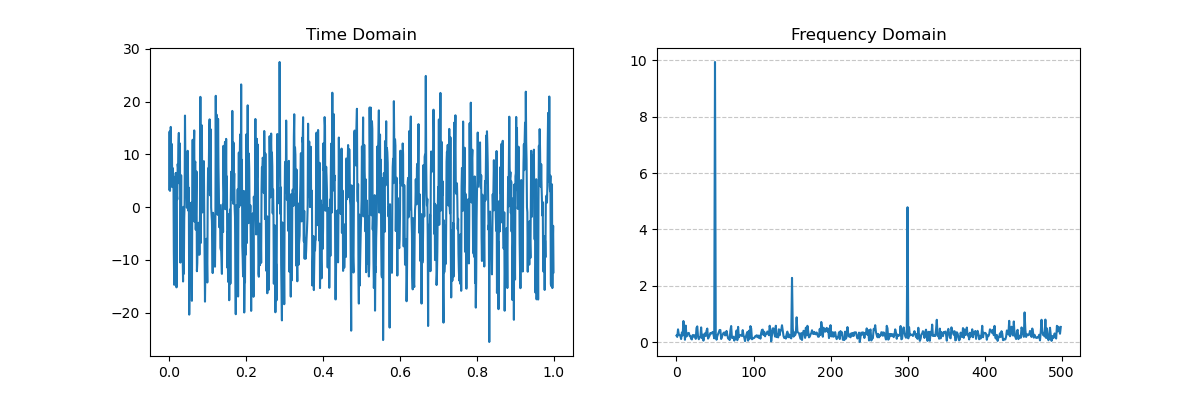
\includegraphics[width=\textwidth]{./images/transform.png}
    \caption{Some signal in the time-domain (displayed on the left) with added noise. Computing the transform with a discrete version of the Fourier transform reveals the main frequencies that make up the original signal in the time-domain (displayed on the right)\label{fig:transform}}
\end{figure}

Even though the Fourier transform is an incredibly powerful function, its formula is compact. 
$$\hat{f}(x) = \int_{-\infty}^{\infty} f(t)e^{-i2\pi x t} dt$$
It is worth noting that \textit{transform} refers to both the act of transforming the function as well as the output of the transform. Additionally, the time-domain to frequency-domain transform is sometimes called the forward transform to emphasize the transformation direction. 

% High level description of the Fourier transform.
\subsubsection{Fourier transform intuition}
For the sake of simplicity, let $f$ be a periodic function with a period of $2\pi$. The following equations help explain how the Fourier transform works.
\[ \int_0^{2\pi} sin(mx)sin(nx)dx = \int_0^{2\pi} cos(mx)cos(nx)dx= 
\begin{cases} % Some issues with cases
    0 & m\neq n \\
    \pi & m=n
\end{cases} 
\]
\noindent and
$$\int_0^{2\pi} sin(mx)cos(nx)dx = 0$$

If $n = m $, $sin(nx), n\in\mathbb{Z}$ will interfere with $sin(mx), m\in\mathbb{Z}$, and integrating over the interval yields $\pi$. If $n \neq m$, integrating over the interval gives 0. When the result of the definite integral is 0, there is no correlation between the two signals. 

Intuitively, the Fourier transform is a function that checks correlation between a signal and all sinusoids. For example, transforming the signal $sin(440t)$, yields a 0 for every sinusoid, except $sin(440t)$, which means that $sin(440t)$ is part of the original signal.

\begin{figure}[ht]
    \centering
    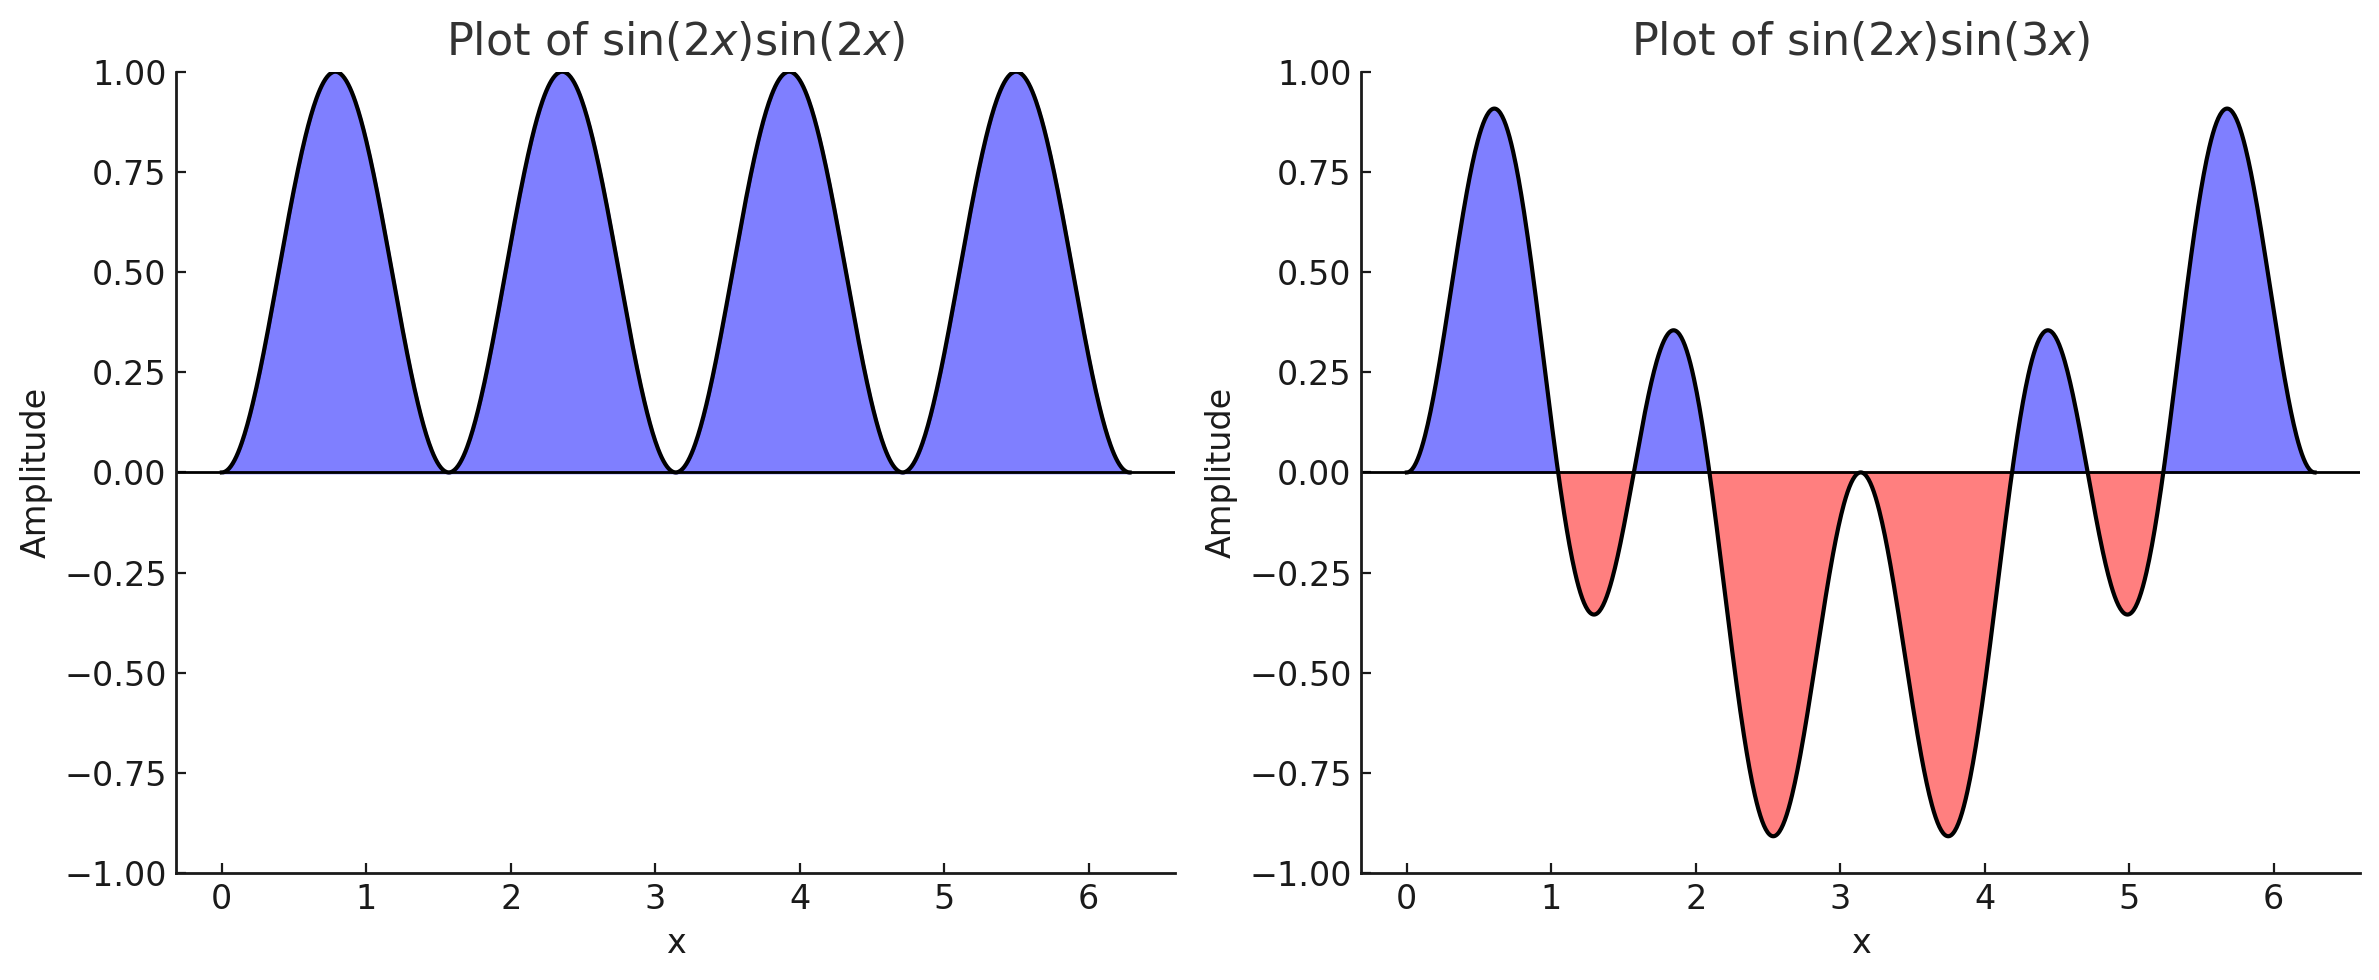
\includegraphics[width=\textwidth]{./images/transformIdea.png}
    \caption{The graphs of $sin(2x)sin(2x)$ and $sin(2x)sin(3x)$ on the $0$ to $2\pi$ interval. Matching $n$ and $m$ results in $sin^2(2x)$ which is always positive, resulting in a positive area whereas a mismatch causes equal positive and negative area, canceling out to 0.\label{fig:transformIdea}}
\end{figure}

% DFT
\subsection{Discrete Fourier transform} 
The Discrete Fourier transform (abbreviated as DFT), as the name implies, is the Fourier transform for discrete signals. Instead of integrating over the entire function domain, the discrete samples from $t=0$ to $t=N$ are summed. The DFT for a signal $x$ with $N$ points is 
$$X_k = \sum_{n=0}^{N-1} x_ne^{-\frac{i2\pi kn}{N}}$$

% Matrix
\subsubsection{Matrix representation for the DFT computations} 
The DFT can be represented and computed by a matrix-vector multiplication. 
$$
% DFT coefficients
\begin{bmatrix}
    X(0) \\
    X(1) \\
    X(2) \\
    X(3) \\
    \vdots\\
    X(n) \\
\end{bmatrix}
=
% DFT matrix
\begin{bmatrix}
    1 & 1 & 1 & 1 & \cdots & 1\\
    1 & \omega & \omega ^2 & \omega ^3 & \cdots & \omega ^n\\
    1 & \omega ^2 & \omega ^4 & \omega ^6 & \cdots & \omega ^{2n}\\
    1 & \omega ^3 & \omega ^6 & \omega ^9 & \cdots & \omega ^{2n}\\
    \vdots & \vdots & \vdots & \vdots & \ddots & \vdots \\
    1 & \omega ^{n} & \omega ^{2n} & \omega ^{3n} & \cdots & \omega ^{{n^2}}\\
\end{bmatrix}
% Discrete signal
\begin{bmatrix}
    x(0) \\
    x(1) \\
    x(2) \\
    x(3) \\
    \vdots\\
    x(n) \\
\end{bmatrix}
$$
where $n = N-1$ as the computation are zero-indexed and $\omega$ is the principle N-th root of unity $e^{2\pi i/N} $. 

% \todo{but why a matrix when the summation formula is both practical and more compact..? Also, FFT? What's the damn point?}

% Inverse transform
\subsection{Inverse transforms}
The time-domain signal can be used, transmitted, and received, but is difficult to to analyze and modify. The frequency domain, in contrast, is easy to analyze and modify, but makes little to no sense in many use cases. For example, a C-major chord in the frequency domain cannot be played. The forward Fourier transform allows the transformation from time to frequency domain, but once any modification (like high frequency filtering) is applied, the signal needs to be transformed back to the time domain to be usable. The operation that does this is appropriately called the inverse Fourier transform, IFT for short or IDFT, for the discrete variant.

The inverse Fourier transform is very similar to the forward Fourier transform:
$$ f(t) = \frac{1}{\pi}\int_{-\infty}^{\infty} \hat{f}(x)e^{i2\pixt} dx$$
and the discrete inverse transform is 
$$ x_n = \frac{1}{N}\sum_{k=0}^{N-1} X(k)e^{\frac{i2\pi kn}{N}}$$

The only difference is a normalization factor and negation of the exponent.

% Computing
\subsection{Computations}
For pretty much any practical usage of the DFT, so many samples will be used that it's not feasible to compute by hand. The DFT computations thus need to be converted to an algorithm or similar programmatic construct a computer can understand and run.

\subsubsection{Example DFT using the formula}
The DFT formula is technically easy to use both in manual computations and when writing software to compute it. Given a discrete input signal 

$$x = [-0.01298834,  0.62287525,  0.64266088,  0.39309558,  0.55407458, \cdots]$$

which has a 100 elements, the DFT values can be computed with the formula $$X_k = \sum_{n=0}^{N-1} x_ne^{-\frac{i2\pi kn}{N}}$$

Starting with $k=0$ $X_0 \approx -0.3215+0i$, a number with both the real and imaginary components close to 0, which indicates very little impact on the original signal. At $k=5$ however, $X_k \approx 0.07725-24.5836i$ with a relatively large imaginary component. Repeating the same summation up to $k=100-1 = 99$ the other values of $X_k$ with relatively large imaginary components are at $k=12$ and $k=25$. 

To obtain the frequency-magnitude plot, which simply will be referred to as the \textit{spectrum} from here on, the magnitudes for each complex valued $X_k$ are needed. The magnitude represents the length of the equivalent vector of the DFT values, and since the vector forms a right triangle, the length of the vector (or hypotenuse of the triangle) can be computed using the Pythagorean theorem $a^2 + b^2 = c^2$. 

% Nyquist thing here

\subsubsection{Computing the DFT programmatically}
As the Fourier transform relies so heavily on complex arithemetic, the effort to implement it largely depends on the features of the chosen programming language. With built-in complex data types and extensive mathematical and scientific computing libraries, implementing the DFT in Python is trivial. Leveraging Python's cmath library, the computations can be copied directly and 2 for-loops handles the summation and $X_k$ indexing as shown below.

\lstinputlisting[style=python]{../snippets/dft-A.py}

For a more primitive language without complex exponentiation like C, the computations are still fairly straightforward to do due to Euler's formula that expands $e^{ix} = cos(x) + isin(x)$. The components can be separated into two separate data structures and so the imaginary unit can be dropped. A possible C implementation (without using a struct for complex numbers) is shown below. 

\lstinputlisting[style=c]{../snippets/dft-A.c}

\subsubsection{Computing the inverse}

Implementing the IDFT in Python is as trivial as the DFT due to the language's features. The similarity in the formulae is reflected in the code, being the same apart from the normalization and negated exponent. 

\lstinputlisting[style=python]{../snippets/dft-C.py}

The inverse may be used after processing the frequency domain. For example,  Figure \ref{fig:DFT-IDFT} shows both a signal and the signal aftering filtering in both time and frequency domain. The method of filtering out noise was simply to remove values under a thresholdin the frequency domain. The IDFT was then used to create a new time-domain signal from the modified frequency domain.

\begin{figure}[ht]
    \centering
    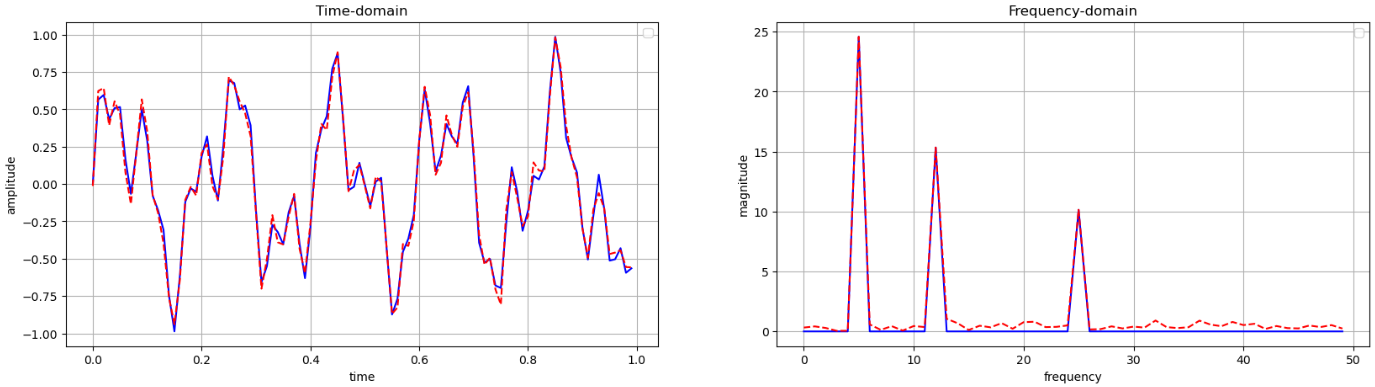
\includegraphics[width=\textwidth]{./images/filtered_signal.png}
    \caption{The time-domain and frequency-domain representations of the signal (red dashed line) and the filtered signal (blue solid line)\label{fig:DFT-IDFT}}
\end{figure}

% FFT
\subsection{Fast Fourier transform}
The DFT takes $n^2$ operations to perform as there are $n$ outputs $X_k$ and $n$ amount of numbers to be summed. A fast Fourier transform (abbreviated as FFT) is any method that speeds up the computation of the DFT. This means that even if there is one Fourier transform and basically one DFT, there are multiple FFT algorithms. Arguably, very few users of the FFT care about the implementation, they just expect the functionality of the DFT, but faster. 

\subsubsection{Time complexity}
The term time complexity refers to the asymptotic performance of an algorithm. Even though it often correlates with performance, it is ultimately theoretical and only considers the highest-order term, because it is the greatest contributor when the input size grows towards infinity. For example, consider an algorithm for multiplying 2 numbers. One such algorithm, commonly taught in elementary school, multiplies every digit of one operand with every digit of the other. The result of each multiplication is added to the previous, accounting for carrying, to form a single number. This process results in an array of numbers, each of which is a multiple of a power of 10. The final step of the algorithm is to sum these numbers. The first step takes $N^2$ operations, where $N$ is the length of the operands (assuming they are the same length), and the second step takes $N$ operations. This algorithm, thus, takes $N^2+N$ steps but as N grows larger and larger, the $N^2$ term will contribute the most, so we say that the algorithm has a complexity of $O(N^2)$, which is referred to as \textit{Big-O}. For example, multiplying two 1000 digit long integers, the multiplication will take a million operations, and the summation will take 1000. Increasing the input size with 1 digit adds only 1 more addition, but it adds 1001 more multiplication steps.

Perhaps the most popular algorithms, the Cooley-Tukey FFT, has an algorithmic complexity of $O(n \log n)$, a significant speedup over $O(n^2)$ \cite{Randhawa2018} \cite{HeidemanEtAl1984}. Once in Big-O, the base of the logarithm does not matter, what matters is that it is logarithmic. An improvement from $O(n^2)$ to $O(n \log n)$ means that even with a mere 1000 samples, the speedup, purely in terms of time complexity, is approximately 100x. In a paper by James Cooley, he exemplified a computation with the Fourier transform on a dataset of 512,000 data points which he claims would see an approximately 12,800x speedup with the FFT \cite{Cooley1987}; 512,000 data points would take on the order of 262 billion operations to complete with an $O(n^2)$ algorithm which, with a modern personal computer, can take minutes to complete. An $O(n \log n)$ algorithm takes a relatively measly 9.7 million operations and runs in milliseconds. This is akin to measuring the execution time of Quick sort to Bubble sort for an array of size 512,000 which indeed sees a speedup of this magnitude.

This speedup in execution time and theoretical time complexity improvement demonstrates the power of the FFT. Why this improvement is so important will, hopefully, be evident later. Essentially, the FFT is considered by some to be one of the most important algorithms of all time due to being able to perform very important heavy computations instantaneously. 

% \subsubsection{Brief history of the FFT} \todo{this whole section is bad, I'll either fix it or remove it later}
% The history of the FFT is long and cloudy with multiple scientists working on a similar problem between 1800-2000. Cooley and Tukey introduced their algorithm in 1965 and at the time it was regarded as a completely new and revolutionizing algorithm. Based on the papers [A] and [B], the FFT and similar numerical methods were developed in two chains. One of them was started with Euler and Lagrange which Gauss based his work on. Runge's work is based on ????????? Gauss and was the basis for a lot of other development. The other chain, which seemingly does not link to Gauss is where Cooley-Tukey exists. They tributed I.J. Good in their paper even though their algorithm was pretty different from the Good one, which is now commonly called the Prime Factor Algorithm and sometimes Good-Thomas. 

% % Yates used? FFT for a convolution

% It was later discovered that Cooley-Tukey works almost exactly as the algorithm Gauss had proposed almost a century earlier. This is probably why Cooley talks about the "re-discovery" in one of his paper. Since the algorithm was only rediscoverd by Cooley and Tukey, some would like to give Gauss more credit for the FFT and some authors have used terms such as "Discrete Gauss Transform (DGT)" and "Gauss-Fourier Transform (GFT)". To make the history of the FFT even muddier, Clairaut published a cosine-only "DFT" 50 years before Fourier even came forth with the Fourier series. Lagrange came up a sine-only DFT-like formula around 40 years before Fourier series.

% At first, the Cooley-Tukey algorithm was regarded as an entirely new thing.   
% The modern FFT (what's that?) is based on the work of Gauss, almost which was developed almost a century before Cooley-Tukey. Gauss and CT use the same algorithm but the equivalence is not obvious due to Gauss' obscure and outdated notation.

% Some would like to credit Gauss with the FFT even though it would be impractical. Some have and there have been uses of the terms "Discrete Gauss transform (DGT)" and " Gauss-Fourier transform (GFT)".

% In the 1800s, an FFT which was NOT based on Gauss was widely used

% Clairaut published a cosine-only "DFT" in 1754, 50 years BEFORE Fourier's Fourier series??? Lagrange came with a sine-only DFT-like formula in 1762


% CT > Good > Thomas, Yates
% Rudnick > Danielson-Lanczos > Runge 
% Gauss > Lagrange, Euler
% Smith > Darwin > Thompson > Runge
% Smith > Everett > Darwin & Smith > Kelvin > Everett > Darwin
% What is the link between Thomas, Yates and the "rest"?
% What's the link between Gauss and Runge
% Where does Carlini fit into the picture?

\subsubsection{The FFT algorithm}
As previously mentioned, FFT is simply put any algorithm that computes the DFT \textit{fast}. One of the easier to understand while still demonstrating the workings of the algorithm is the Radix-2 FFT. The Radix-2 FFT is easy to understand because it assumes the input size is a power of 2, meaning it is easy to recursively split into two. On a high level, the Radix-2 algorithm starts with splitting the input array into odds and evens. It then calls itself for the odds and evens, recursively splitting the array until it performs FFTs on arrays of length 1. On the way back up, it performs the DFT on smaller units of the original signal, utilizing the symmetry of roots of unity and values that it has already computed to perform multiple operations at once. 

The following mathematical derivation of the Radix-2 FFT is adapted from \cite{Rozman2019}. It starts with splitting the DFT into two sums, one for the even indices and one for the odd 
$$X_k = \sum^{N/2-1}_{n=0} x_{2n}T^{2n}+ \sum^{N/2-1}_{n=0} x_{2n+1}T^{2n+1}$$
where $T_k$ is called the twiddle factor $e^{-\frac{2\pi ik}{N}}$. A common twiddle factor is factored out of the odd sum and the even and odd sums are denoted as $E_k$ and $O_k$ respectively. 

$$X_k = E_k + T_kO_k$$

These functions $E_k$ and $O_k$ are periodic with a period $N/2$ which can be shown by showing that $$e^{\frac{-2\pi in(k+N/2)}{N/2}} = e^{\frac{-2\pi in(k)}{N/2}}$$
which means that 
$$E_k = E_{k+\frac{N}{2}}, O_k = O_{k+\frac{N}{2}}$$
and since this holds true for $E_k$ and $O_k$, the following is also true

\[
X_k = \left\{\begin{array}{lr}
    E_k + T_kO_k, & \text{for } 0 \leq k < N/2\\
    E_{k-N/2} + T_kO_{k-N/2}, & \text{for } N/2\leq k< N\\
    \end{array}\right\}
\]

This means that the DFT can be computed in two layers (for lack of a better term), the lower $N/2$ terms and the upper $N/2$ terms.
When computing the upper $N/2$ terms, i.e. when $N/2 \leq k < N$, $X_k = E_{k-N/2} + T_k^{N/2}O_{k-N/2}$, which are the same O and E as the lower $N/2$ terms, just with an offset of N/2. The twiddle factor is raised to the power of N/2 because it too is in terms of $k$. We can thus split $X_k$ into 
% \todo{This section could be reworked}

$$X_k = E_k + T_kO_k$$  
$$X_{k+N/2} = E_k + T_k^{N/2}O_k$$
which are the equations for the lower and upper $N/2$ terms. Finally, the twiddle factor is rewritten using the following property of complex exponentials

$$e^{\frac{-2\pi i(k+N/2)}{N}} = -e^{\frac{-2\pi ik}{N}}$$
which gives

$$X_k = E_k + T_kO_k$$  
$$X_{k+N/2} = E_k - T_kO_k$$

Recall that

$$E_k = \sum^{N/2-1}_{n=0} x_{2n}T_k^{2n}$$
$$O_k = \sum^{N/2-1}_{n=0} x_{2n+1}T_k^{2n}$$
and that the DFT is
$$X_k = \sum^{N}_{n=0} x_nT^{n}$$

The similiarity of the formulae implies that when the element indices are adjusted, $E_k$ and $O_k$ are both DFTs essentially. To transform this purely mathematical notation into a working program, the core computations are implemented with a loop

\begin{lstlisting}
do k = 0, N/2-1
    T = exp(-2*i * PI * k / N) 
    X(k+1) = E(k+1) + T * O(k+1)
    X(k+1 + N/2) = E(k+1) - T * O(k+1)
end do
\end{lstlisting}

In Fortran, arrays are indexed starting from 1, this means that every array access needs an offset of 1. Before these computations, the evens and odds must be computed.

\begin{lstlisting}
E = r2fft(input(1:N:2))
O = r2fft(input(2:N:2))
\end{lstlisting}

Any recursive algorithm also needs a base case to prevent the algorithm from looping indefinitely. In the case of the FFT, this is when the input array has a single value.

\begin{lstlisting}    
if (N == 1) then
    X = input
    return
end if
\end{lstlisting}

Putting everything together and adding variable declarations and initialization as well as the function declaration, a naive Radix-2 FFT could look like the following

\lstinputlisting[style=fortran, label={code:fortran-fft}]{../snippets/fft-A.f90}

This implementation assumes the input is a power of 2, but this is not handled anywhere. The program still runs, but gives an erroneous answer. The algorithm can be visualized with a block diagram as shown in Figure \ref{fig:FFT-Alg}.

\begin{figure}[ht]
    \centering
    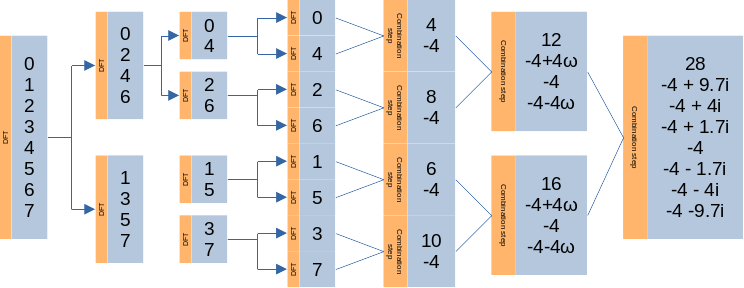
\includegraphics[width=\textwidth]{./images/fft.png}
    \caption{Diagram of a 4-point FFT. The process starts with splitting down the input vector to the recursive base case $N=1$. After that the values are combined using the core computations of the FFT.\label{fig:FFT-Alg}}
\end{figure}

\subsubsection{Time Complexity of Radix-2 FFT}
The FFT is ubiquitous, and the algorithm has been explored extensively. Literature explaining and deriving the algorithm exists and following it to implement the algorithm in code is almost trivial. It is easy to overlook the ingenuity of the algorithm considering the simplicity of it when seeing it written down. Where the $O(n\log n)$ complexity comes from might not be entirely clear even when seeing the algorithm written out in code because, even though the divide-and-conquer method recursively splits the array, multiple computations are done within each function call. 

When taking a 4-point FFT, as shown in Figure \ref{fig:FFT-Alg}, the last combination step definitely needs four computations. It can also be observed that each of the 2-point FFTs (which is a subproblem of the 4-Point FFT) takes 2 computations. All in all, it takes eight computations to compute the 4-point FFT. The total number of computations for an 8-point FFT similarly is 8 plus 2 * number of computations of the 4-point FFT. As the FFT is a recursive algorithm, the total number of computations for an N-point FFT can be generalized to the following recursive formula
$$T(N) = 2*T(N/2) + N$$
where N is assumed to be a power of 2, for simplicity. This recursive definition can be expanded
until we get the recursive base case T(1). Since N is halved for every step, it takes precisely $\log_2 N$ expansions to reach the base case. Expanding the definition a few times (assuming N is sufficiently large)
$$T(N) = 2*(2*T(N/4) + N/2) + N = 4*(T(N/4) + N) + N$$
$$= 4*((2*T(N/8)+N/4) + N) + N = 8*T(N/8) + N + N + N$$
$$= 8*(2*T(N/16) + N/8) + N + N + N = 16*T(N/16) + N + N + N + N$$
reveals the pattern $T(N) = 2^k*T(\frac{N}{2^k}) + kN$, where $k$ is the number of times the recursion is expanded to reach the base case. As $k =\log_2(N)$, the formula becomes $T(N) = 2^k*T(\frac{N}{2^{\log_2(N)}}) + kN$ which equals $T(N) = 2^k*T(\frac{N}{N}) + kN = 2^k * T(1) + kN$. As the 1-Point FFT performs no computations, $T(1) = 0$ and the final formula for the total number of computations for the N-point FFT is $N \log_2(N)$. In the context of Big-O, it only matters that the algorithm is logarithmic, the base will not matter in the same way that constants and linear scalars are dropped. This gives the well known $O(N\log N)$.

\subsubsection{Inverse FFT}
The inverse of the FFT, or IFFT, is nearly identical to the FFT algorithm. Like the IDFT bonly adding normalization and negating the exponent, the IFFT is the FFT  with $\omega = \frac{1}{n}e^{\frac{i2\pi kn}{N}}$. In other words, the IFFT is the FFT with a negated exponent, and a normalization added. In \cite{Reducible2020} it is shown that the IFFT algorithm can reuse the FFT logic, with a single line changed. 

The Fortran code from earlier contained a inverse factor that was left unexplained. Below is an example of a simple abstraction for calling the forward FFT and inverse FFT but utilizing the same core r2fft function.

\lstinputlisting[style=fortran]{../snippets/fft-B.f90}

Both the FFT and inverse FFT are utilizing the same core Radix-2 implementation from earlier, but the inverse is computed with a negated twiddle factor based on the second argument. In the inverse FFT case, an additional normalization is also applied after the FFT computations are finalized.

This implementation can be tested empirically by first forward transforming a set of data points and then inverse transforming the transform and note that $x = ifft(fft(x))$ holds up to floating-point precision. When comparing $a$ and $b = ifft(fft(a))$, all values were within $\epsilon = 1*10^{-30}$ when using quadruple-precision floating point variables and data structures.

Fortran is one language that has native complex arithmetic making it a very convenient language to implement complex number related algorithms in. In a language like C or JavaScript without such functionality, one way is to take the complex conjugate of the input, which is effectively equivalent to negating the twiddle factor. This can be verified using Euler's formula $e^{ix} = \cos(x) + i\sin(x)$. Cosine being an even function and sine being an odd function means that $e^{-ix} = \cos(-x) + i\sin(-x) = \cos(x) - i\sin(x)$ which is the complex conjugate of $\cos(x) + i\sin(x)$. 

% Applications 
\subsection{Applications of Fourier analysis}
Fourier series were originally motivated by a differential equation in physics and even if it still is of great help for mathematicians solving similar problems, the true importance comes from the vast applicability of Fourier analysis combined with the significant performance improvement of the FFT. The Fourier transform allows the conversion between time and frequency domain which makes manipulation and analysis of arbitrary signals practical. 

Signals are all around us, hidden in every day life. Merely accessing the internet using a wireless connection most likely involves the Fourier transform. The following chapter will briefly explore some of the applications of the Fourier transform to emphasize the importance of the idea. 

% \todo{https://warse.org/IJWCNT/static/pdf/file/ijwcnt04332014.pdf}

\subsubsection{Wireless communication}
Several modern standards for wireless communication, like IEEE 802.11 WLAN (colloquially Wi-Fi), rely on Orthogonal Frequency Division Multiplexing (OFMD) \cite{GnanishivaramNeeraja2014}. In short, OFMD is a way to pack discrete data (consecutive bits, for example) compactly into a time-domain signal of orthogonal sinusoids. Orthogonal means that the signals do not interfere with each other and that integrating the product of several sinusoids over the period gives 0. This happens to be case when the angular frequency of two signals are two different integers. 

OFDM needs a modulation scheme to convert data into sinusoid components. Quadrature Phase Shift Keying is one popular method, and it transforms the 4 combinations of 1's and 0's into 4 complex numbers, $\pi/2$ radians apart. There are different ways of assigning the values, for example, 00 may become 1, 01 becomes i, 10 becomes -1 and 11 becomes -i. These values are encoded in subcarriers which are then turned into the time domain using the IFFT in preparation for transmission. An FFT on the receiver's end transforms the transmission into frequency domain for demodulation. The frequencies and phases can then be extracted using the inverse of the modulation scheme to obtain the original data that made up the transmitted time-domain signal.

\subsubsection{Multiplication}
% \todo{This whole section may be wrong as I delved deeper into the FFT algorithm after I wrote this}
The FFT can be used to multiply two numbers, which after building a good understanding of the FFT, may feel wrong to someone learning about it. Not only can it perform multiplication, it can increase the efficiency of it. Multiplication is an algorithm that has a time complexity of $O(n^2)$ because each digit needs to be multiplied by every other digit. Using a fast Fourier transform, two numbers can be multiplied in $O(n \log n)$. The general gist of the method is to represent both numbers as polynomials, sampling them at a number of points, a number which must be large enough to uniquely define the polynomial, multiplying those points together, finding a new unique polynomial for the new set of points and converting the polynomial back to a number. That resulting number is the product of the two input numbers \cite{Reducible2020}.

Sampling means that the polynomial is evaluated at some points. A polynomial in coefficient form can be written like $P(x) = \sum^d_{n=0} a_nx^n$. If the polynomial is evaluated at $\omega = e^{-\frac{i2\pi k}{N}}$, the resulting expression is $\sum^d_{n=0} a_n(\omega)^n = \sum^d_{n=0} a_ne^{-\frac{i2\pi k n}{N}}$ which is the DFT definition, where $a$ is a discrete input signal with $d$ points. This means that the DFT is evaluating a polynomial at the nth roots of unity, which also means that the FFT can evaluate a polynomial at the nth roots of unity \cite{Emerencia2007}.

Even though this proposed method for multiplication seems like a very convoluted process, for large numbers, this turns advantageous at inputs of length around 200 \cite{Emerencia2007}. This means that the method is practical in cryptography where it is fairly common to multiply extremely large integers. 

In practice, it is not a trivial method to implement. The FFT (and IFFT) does indeed just work, but only for polynomials. The difficult part is converting back and forth between polynomial and integer. Each coefficient in a polynomial represents a digit in the integer, yet coefficients are not limited to the digits 0-9. There are multiple ways to do this conversion and one way involves modular arithmetic in conjunction with long addition. This method does not work for negative numbers, but an easy circumvention is to force both inputs to be positive and simply noting whether the output is negative. This can be done by checking if exactly one of the inputs is negative, in which case the output is negative.





 

\section{Fourier transform applications}
Fourier series were originally motivated by a physics differential equation and even if it still is of great help for mathematicians solving particular types of differential equations, the true importance comes from the vast applicability of Fourier analysis combined with the significant performance improvement of the FFT. The Fourier transform allows the conversion between time and frequency domain which makes manipulation and analysis of arbitrary signals practical. 

Signals are all around us, hidden in every day life. There are the more obvious ones like various forms of sound and wireless communications that everyone with a mobile phone utilizes multiple times per day. There are also less obvious ones like images and really any kind of data. This chapter will explore some of the applications of the Fourier transform to emphasize the importance of the idea. 

\subsection{Wireless communication}
A lot of modern standards for wireless communication, like IEEE 802.11 WLAN (colloqially Wi-Fi), rely on Orthogonal Frequency Division Multiplexing (OFMD) \todo{https://warse.org/IJWCNT/static/pdf/file/ijwcnt04332014.pdf}. In short, it's a way to pack discrete data (consecutive bits for example) compactly into a time-domain signal of orthogonal sinusoids. Orthogonal means that the signals do not interfere with eachother and that integrating the product of several sinusoids over the period gives 0. This happens to be case when the angular frequency of two signals are two different integers. \todo{Source? Even though some literature and sources just take this for granted. When n = m, the integral is $sin^2(nx)$ which will always be positive so the integral is not 0.}

OFDM needs a modulation scheme to convert data into sinusoid components. Quadrature Phase Shift Keying is one popular method and it transforms the 4 combinations of 1's and 0's into the 4 roots of unity. 00 becomes 1, 01 becomes i, 10 becomes -1 and 11 becomes -i. These values are encoded in so called subcarriers which are then turned into the time-domain using the IFFT in preparation for transmission. An FFT on the receiver's end transform the transmission to frequency-domain for demodulation. The frequencies and phases can then be extracted using the inverse of the modulation scheme to get the original data that made up the transmitted time-domain signal.\todo{Source?}

% \subsection{Spectroscopy}

\subsection{Images are signals}
Just like data is encoded in a signal for wireless communication, a signal can be also used to represent an image. Optical illusions show that human  eyes are not great at spotting certain information. The lossy image format JPEG uses this to it's advantage, getting rid of small color changes, while keeping high contrast brightness changes.  

The Discrete Cosine Transformed  is typically the preferred method for it's properties aligning closer to the goals of image processing and because it's simpler to compute, being limited to real inputs and outputs \todo{does the DCT need a source?}. However \todo{there is one paper that uses the FFT specifically, need to look into what makes it special there, or not?}

\subsection{Multiplication}\todo{This whole section may be wrong as I delved deeper into the FFT algorithm after I wrote this}
A more novel example of an application of the FFT is the multiplication of two numbers. As previously mentioned, multiplication is an algorithm that has a time complexity of $O(n^2)$ because each digit needs to be multiplied with every other digit. Using a fast Fourier transform, two numbers can be multiplied in $O(n \log n)$. The general gist of the method is to represent both number as a polynomial, sampling them at a number of points (a number which must be large enough to uniquely define the polynomial), multiplying those points together, finding a new unique polynomial for the new set of points and converting the polynomial back to a number. That resulting number is the product of the two input numbers \cite{Reducible2020}.

Sampling is where the FFT enters the picture. The last step of the multiplication method requires a unique polynomial so $N \geq d+1$ samples are necessary where $d = n-1$, the highest degree in the polynomial or one less than the number of digits in the inputs. For every sample, the entire polynomial is required which means that the sampling part takes $O(n^2)$ computations anyway. The FFT accelerates this by utilizing the symmetry in the roots of unity to take the samples in $O(n \log n)$. This procedure is done for both input numbers, contributing $2n \log n$ operations or $(n \log n)$ \cite{Reducible2020}.

The next step is a component wise multiplication of the transforms, which takes $O(n)$ operations. The last step involves taking the inverse to get the result. This is done with the inverse FFT, which also runs in $O(n \log n)$ \cite{Reducible2020}.

All in all the multiplication algorithm takes $4N + 3(n \log n)$ operations which is $O(n \log n)$. Even though this seems like a very convoluted process, for large numbers, this turns advantageous at inputs of length around 200 \cite{Emerencia2007}. This means this method is practical in cryptography where it's somewhat common to multiply extremely large integers. 



\subsection{Music and audio processing} 

% Body

\section{ Using short time Fourier transform for pitch detection}
The purpose of this work is to study a short-time Fourier transform for its viability as a pitch detector. The FFT for transforming a waveform into the frequency-domain has been introduced and this chapter will focus on the properties of sound, introduce some musical terminology and how the FFT can be used to detecting pitches from a time-domain signal

\subsection{Basics of sound}
Sound physically is pressure propagation through a medium, a vibration which some things can produce, and some things can pick up. The word sound can be used to describe both the propagation itself and the phenomenon we feel when our ears react to the propagation. Headphones, strings of a guitar and vocal chords (together with the lungs) are some of the things that can produce sound and microphones and membranes in ears are things that can pick up sound. The propagation will have a certain strength at some point in the medium it travels through, which can be measured. This allows us to model sound as pressure over time. At time $t$, the pressure at some point can be denoted as $f(t)$. This function over time can also be called a signal.

% source: https://api.pageplace.de/preview/DT0400.9781292055152_A24617782/preview-9781292055152_A24617782.pdf The Science of Sound - Rossing, Moore, Wheeler

One of the simplest ways to generate a sound is connecting a speaker to a device that generates an analog current in the shape of a wave. The current moves an electromagnet which moves a membrane at the same frequency as the generator causing the pressure difference around the membrane. This membrane displaces air at some rate which ears pick up as sound. For example, if the generator produces a 440Hz signal, the speaker's membrane will displace air at the same 440Hz. This displacement is propagated over air and is sensed by our ear as a pitch we call A4. Interestingly, the purity of the signal makes it sound harsh, and it is noise in the signal that gives warmth and beauty to the note. This can be observed in Figure \ref{fig:pianoWave} where the signal (sound made by an electric piano) largely matches a pure A4 (440Hz sinusoid) but not quite. The warmth and beauty is formally called timbre and it allows us to distinguish an A4 on a piano from an A4 on a guitar even though both are A4 sounds.

%https://eprints.hud.ac.uk/id/eprint/17816/1/Final_Thesis_-_November_2012.pdf why is this here?

\begin{figure}[ht]
    \centering
    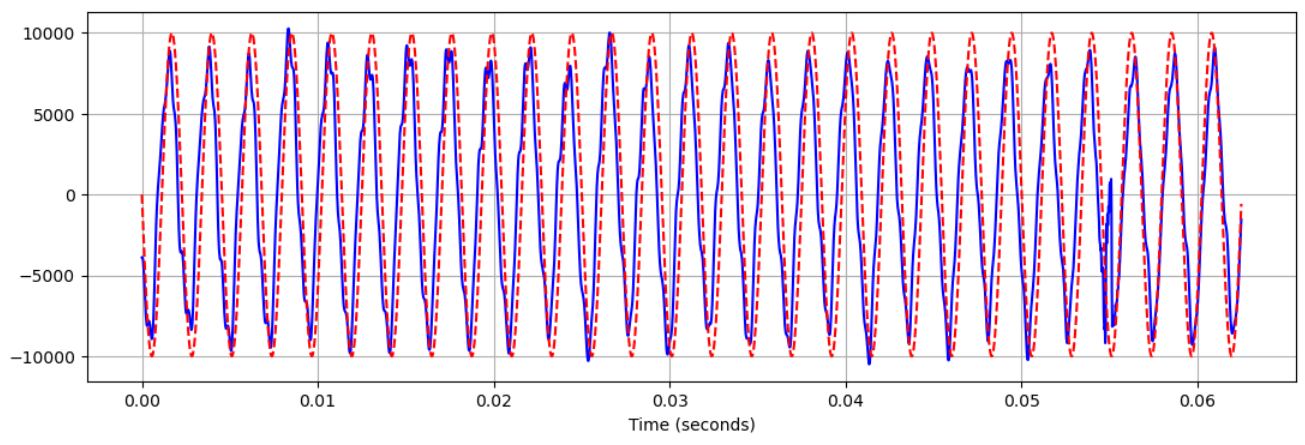
\includegraphics[width=\textwidth]{./images/piano_wave.png}
    \caption{A slice of the recording of a A4 note played on a Yamaha electric piano (blue solid). The signal contains a lot of irregularity but also clear regularity which becomes more evident when layering a pure A4 note on top (red dashed).\label{fig:pianoWave}}
\end{figure}

The characteristics of the sound being played become even more evident when it is converted to the frequency domain through the FFT, as shown in Figure \ref{fig:pianoFreq}. It reveals that, not only is the sound definitely an A4 note due to the overwhelming amount of the 440Hz signal present in the sound, but also what other frequencies contribute to the sound of that piano. 

\begin{figure}[ht]
    \centering
    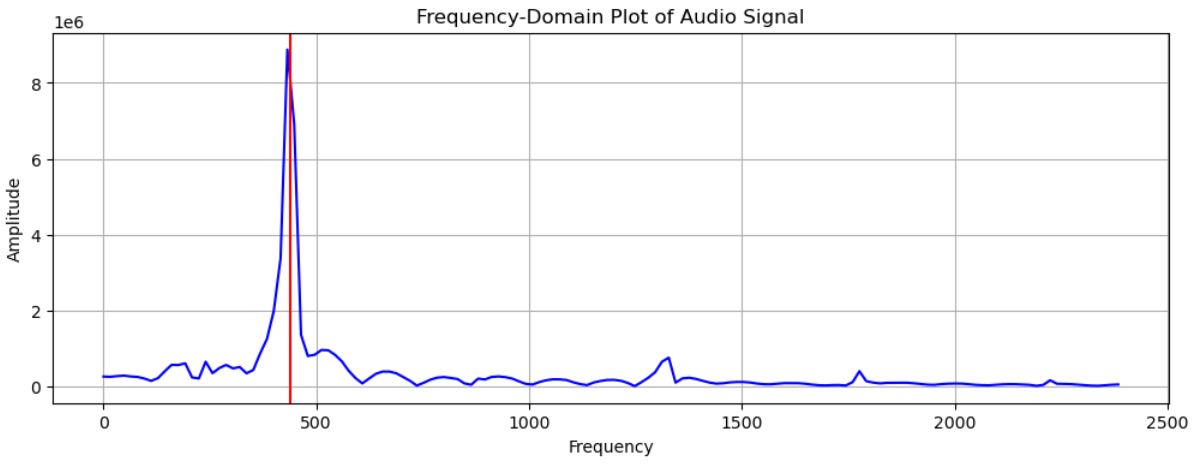
\includegraphics[width=\textwidth]{./images/piano_freq.png}
    \caption{The frequency-domain clearly reveals without any guesswork that the signal is a 440Hz signal with some sort of noise/disturbance. The red vertical line is placed at $x=440$ to show that the peak is the expected 440Hz frequency component.\label{fig:pianoFreq}}
\end{figure}

The spectrum also reveals that the particular electric piano that was used to create the sound lacks harmonic content. This is not the case for  

\subsection{Music 101} 
Music terminology can be hard to define without circular definitions. There's also quite a bit of overlap with the same word meaning different things depending on context. A possible starting point would be defining the octave which is the difference between two sounds where one sound has twice the frequency of the other and is the largest interval in western music. If a sound oscillates at 440Hz, the sounds corresponding to 220Hz or 880Hz are an octave away.


\subsubsection{Octaves}
The name octave comes from the fact that it contains seven distinct basenotes (the 8th forming the octave). This is called a heptatonic scale and when it sounds \textit{nice}, it is called a diatonic scale (formally, it requires a certain structure of intervals). Diatonic scales include the familiar major (happy) and minor (sad) scales. The history and reasoning for the heptatonic scales in western music theory is not relevant for the work, but the point is that it is not the only taxonomy for notes. 

Because the diatonic scales require a certain structure of intervals, the octave needs to be divided further into what is called semitones. Semitone is typically defined as the smallest interval in western music and is typically 1/12th of an octave. Semitone is sometimes also used to talk about, not the interval, but the sounds that bound the interval. This non-interval semitone is sometimes also called a pitch and sometimes note.

\subsubsection{Notes and note names}
Whle octave is used to describe an interval of 2 notes, we can define a first, second third etc. octave if we start from somewhere. A common way to label musical pitches is to use a letter to represent the note name and a number to indicate which octave it belongs to. This system is called Scientific Pitch Notation (SPN) and is used in Western music notation." It starts, not on an A, but on a C and depending on the convention used ends in either a B or an H. Figure \ref{fig:noteScale} shows the octave bounds and how notes are ordered within the octave.

\begin{figure}[ht]
    \centering
    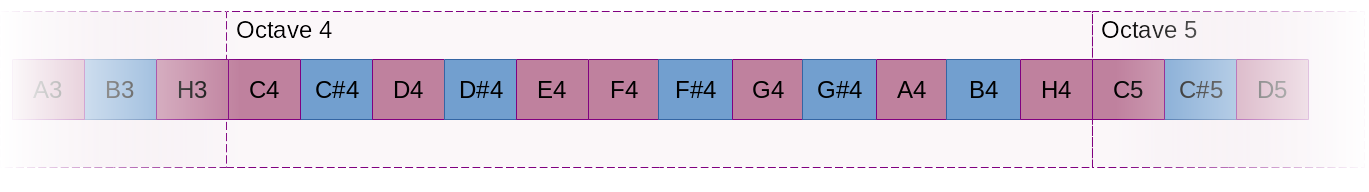
\includegraphics[width=\textwidth]{./images/noteScale.png}
    \caption{Notes of an octave. Base notes are marked with purple. \label{fig:noteScale}}
\end{figure}

For example, the note which has twice the frequency of A4 forms an octave with A4. As the frequency is doubled, the other note is one octave higher than A4 so it is given the name A5. If the frequency is halved, it is named A3. 

In western music, tuning typically starts from A4, which is defined in this system to have a frequency of 440Hz, and every other note is derived from there. Tuning in this context essentially means finding the frequencies of the other notes so that everything sounds \textit{right} (to avoid getting into unnecessary amount of music theory). A3, an octave lower than A4, will be half of 440Hz or 220Hz and A5, an octave higher, will be double of 440Hz or 880Hz. The frequency for the other pitches can be approximated with equal temperament tuning, meaning that all semitones are equally spaced within octaves. This means that the frequency of any one pitch is exactly $2^{1/12}$ times the frequency of the previous one. Sounds are given identifiers as a letter-number pair based on the octave they are in and their placement within the octave. 

\subsubsection{Flats and sharps}
Flats and sharps are augmented notes. Sharps are denoted with a $\#$ symbol and flats with a $\flat$ symbol. Both flats and sharps are one semitone above the augmented note meaning there is quite a bit of overlap. For instance, a D$\#$4 has the exact same pitch as a E$\flat$4. The key difference between D$\#$4 and E$\flat$4 is context. It should be obvious, even to a person with no musical training, that when "playing in D-sharp", there should be a D-sharp and not an E-flat even though they are effectively the same note. In some situations there is also the concept of a "double sharp" and "double flat".    

\subsubsection{Terminology for readers}
The base notes will be defined according to German/EuropeaFusingn music theory as \[C, D, E, F, G, A, H\] and B being $H\flat$. In this work, the term "note" will be used to describe the 12 distinct sounds within the octave because for the pitch detector, discerning the base notes and the sharps and flats isn't necessary. Pitch will be used to describe the measurement/perception of how low or high a sound is.

\subsubsection{MIDI numbers}
For humans, it is easy to use the SPN labels for notes. C4 is a simple pair of a letter and a number and gives users just enough information to know what it refers to. Computers on the other hand are different and instead have it much harder to analyze, say, "A4" even compared to the pure frequencies. However the frequency value is often unnecessary because we usually only care about a discrete set of frequencies corresponding to notes, not all possible real valued frequencies. 
Musical Instrument Digital Interface (MIDI) is a technical standard for protocols, connectors and interfaces relating to music and provides among other things, simple integers for labeling notes. For instance, the first sound on a piano, A0, has the MIDI number 21. 


% \subsubsection{Pitch perception}
% Even though we can clearly define any one pitch to be some frequency, human ears are more complex. 
% What do I want to establish in this chapter????
% What is pitch perception at a high level
% 
\subsection{Fundamental frequency estimation}
Even though we can define a pitch to be a precise frequency, pitch is more of a sensation perceived by ears and we can distinguish pitch from soundwaves that are not simple oscillations. As shown in \ref{fig:pianoWave}, what we perceive as an A4 can contain a lot of noise. As it can be difficult to strictly define pitch, pitch detection may also be hard to define. Pitch is however strongly tied to the fundamental frequency, which is the lowest perceived harmonic of a signal. Even though the timbre of a piano and a guitar are vastly different, which allows us to hear a difference between the two, if they play the same note, the fundamental frequency will be the same. 

From a computational perspective, a possible definition is that pitch detection is the identification of the fundamental frequency and which is the corresponding note (because the sound names are more valuable to musicians than the frequencies expressed as hertz). 

The fundamental frequency is typically the lowest frequency of a signal, but in some cases we can hear a fundamental frequency that isn't actually a part of the signal, a phenomenon appropriately called the missing fundamental. \todo{source: Gotsopoulos}. An example of this would be telephones, that could not record below 300Hz. Male voices would still sound male, even though their fundemental frequency of around 150Hz was completely missing \todo{Mather 2006}.

\subsubsection{The missing fundamental}
The missing fundamental is in a sense an audiotory illusion. It is a result of the constructive interference of harmonics that causes peaks with a period that is the greatest common divisor of the angular frequencies of the harmonics. This is shown in Figure \ref{fig:missingfund} where the sum of several waves produce a wave with a prominently 110Hz oscillation. Even though the lowest frequency component is 220Hz, the prominent 110Hz oscillation is what we feel and hear.

\begin{figure}[ht]
    \centering
    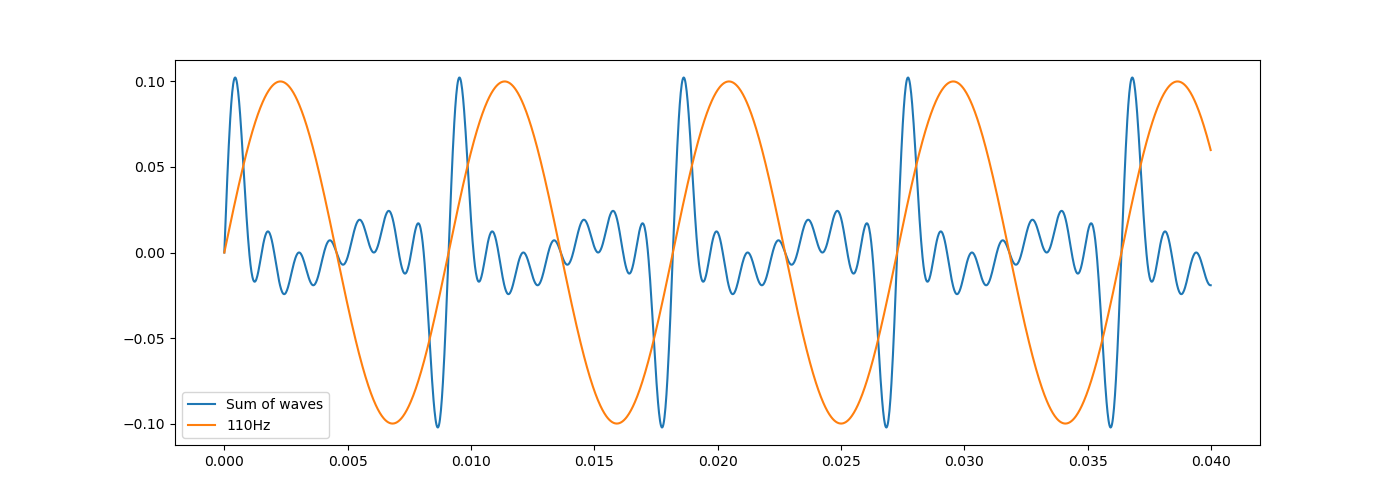
\includegraphics[width=\textwidth]{./images/missingfund.png}
    \caption{Constructive interference of harmonics creates the missing fundemental. Even though the blue signal only contains sinusoids with frequencies greater or equal to 220Hz, the most prominent part of the final signal has a period of 110Hz. \label{fig:missingfund}}
\end{figure}

Pipe organs use this to their advantage. Creating extremely low sounds requires enormous pipes. Taking advantage of the missing fundamental allows relatively smaller organs to produce low sounds.
% 0:56; https://www.youtube.com/watch?v=Sn07AMCfaAI&t=1169s

\subsection{Pitch detection methods}
Pitch detection methods typically fall into one of 3 categories: time-domain, frequency-domain and statistical/machine learning methods. Some common time-domain methods include zero-crossing rate and autocorrelation. Zero-crossing rate, is a method in which frequencies are extracted by keeping track of the rate at which the signal crosses the y-axis. Another is autocorrelation, in which the signal is compared to itself with a different phase. 

This thesis will focus on the frequency-domain approaches, where a fourier transform is used to create a representation of the sound that is easier to analyze and process.

\subsection{Transforming to frequency-domain}
The first step in detecting pitch using a frequency-domain approach is to transform the original signal into the frequeny-domain and there are multiple ways to achieve that. The DFT and FFT were already introduced in the introductory fourier analysis chapter and as already established, some FFT should be used as the transformer as the DFT has terrible performance. How to apply the FFT isn't yet clear however, as the background used dummy data to demonstrate the algorithm and its performance. Disregarding the question of how to process binary audio files, even if the data was decoded, how should the data be processed? If the whole audio signal is given to the FFT, the spectrum will be a complete mess because real music/song contains more than a single note or chord.

\subsubsection{Short-time Fourier Transform}
The short-time Fourier Transform (STFT), sometimes also called the windowed Fourier transform, is a method of analysing a signal by looking at parts of the signal. The STFT is typically defined very similarly to the FT/DFT only with a windowing function applied. The continuous STFT is usually defined like the following.
$$S(x(t), \tau, \omega ) = \int_{-\infty}^{\infty} x(t)W(t-\tau)e^{-i\omega t}$$

where $x(t)$ is the input signal $\tau$ is the center of the window function $W$. The window function may be freely chosen and examples include Gaussian window and Hamming window. Conceptually this is computing the transform for a signal $S_2$ that is some signal $S$ with a windowing function applied so that outside the window, the signal has 0 value. Afterwards, the window is moved and the "next" value is computed. The discrete STFT conversely computes the DFT for just some chunk of a discrete signal. Like the STFT, it then moves the window over some number of steps (called the hop length in discrete context) and repeats. If the hop length is shorter than the window size, the windows will overlap.

This sliding window introduces a new dimension to the output data, a time axis. This data constitutes a spectrogram and the typical way to visualize this data is with a heat map by compressing the 2D of the frequency-domain to a column where intensity represents the magnitude value for a frequency. 

\begin{figure}[ht]
    \centering
    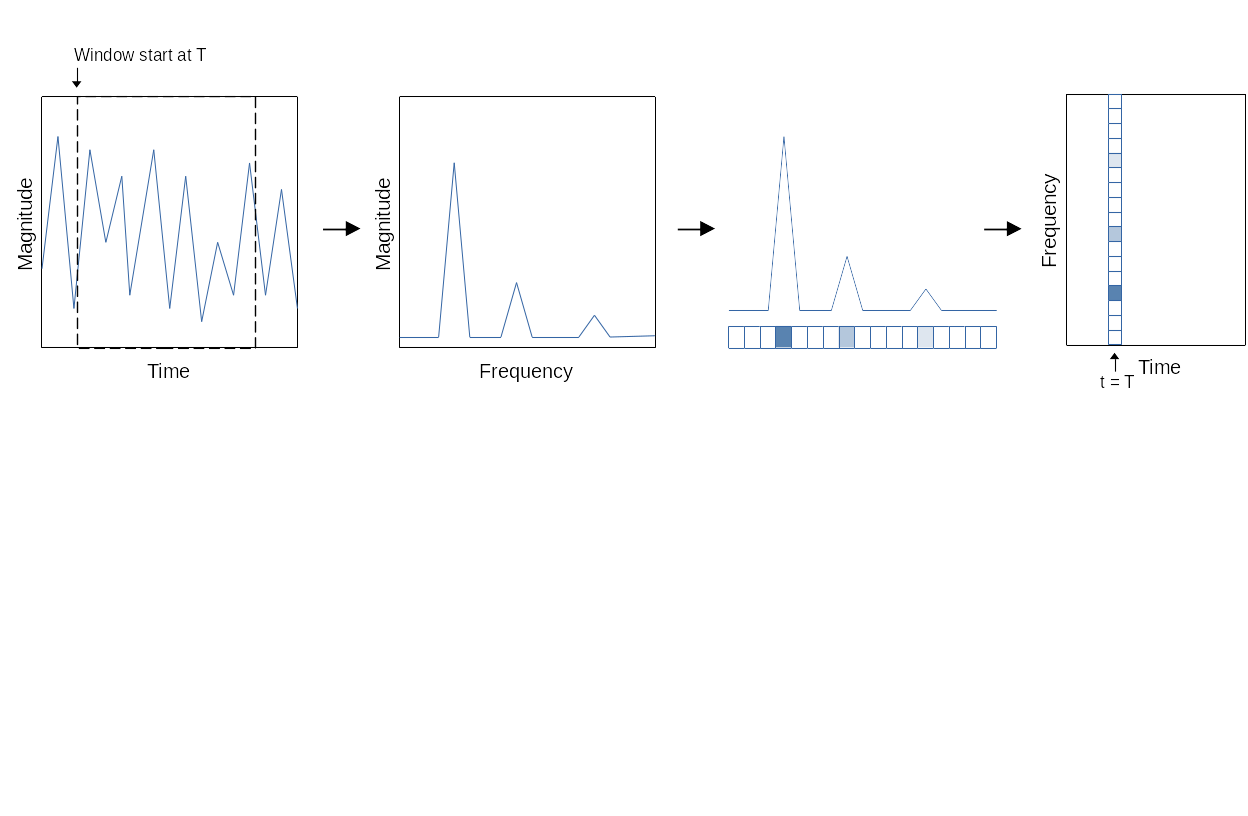
\includegraphics[width=\textwidth]{./images/stft.png}
    \caption{High level overview of the SFTF. The STFT performs the DFT for every window which results in a spectrogram. For ease of visualization, the frequency-domain is typically visualized using color intensity for the magnitude. \label{fig:stft}}
\end{figure}

It is worth pointing out that the STFT is not a special kind of fourier transform, but rather a method of applying the DFT/FFT (or contiunuous FT). This means it has the same behaviour but also that it has the problems which will be introduced shortly. 

For real-time processing, it is both imperetive and a bit redundant to talk about the STFT because the entirety of the signal will never be available so there is no need for windowing. The data will be available as a stream (or chunks) and an FFT can be performed once a buffer is filled, after which the buffer is cleared. The buffer serves as the window so as long as the transform is computed sufficiently often (which needs to be done either way in real-time applications) the method in a sense implements a discrete STFT. The overlap, which is determined by the hop length, doesn't seem to be of much importance for the purpose of the estimation the fundamental frequency and makes little sense when the data becomes available with time. The overlap is important when considering note lengths and separation of repeated semitones \cite{Evans2012}, but does not seem to be a concern for just pitch detection. The pitch detector will thus have a hop length the size of the window, or in other words, no window overlap.

\subsection{Picking peaks from the spectrum}
The Fourier transform is used to get the spectrum data, which can be used to plot which frequencies are part of the original signal. These frequencies that are part of the signal are called partials. Intuitively, for a lot of signals, anyone can look at the frequency-magnitude plot and point to a peak and claim that it is the fundamental frequency and probably be right. Perhaps they are looking for some periodicity with the largest peaks (if there are multiple) and choosing out of those the peak that has the lowest frequency. This is a very straightforward approach and correct for some signals. 

% HPS
\subsubsection{Harmonic Product Spectrum}
Harmonic Product Spectrum (HPS) is an algorithm that almost does the intuitive approach. 
$$Y = \prod_{r=2}^R X_r$$ where $X_r$ denotes the signal $X$ downsampled by $r$. Simply put, the HPS iteratively multiplies downsampled version of a signal. Downsampling the frequency-domain effectively compresses the frequency-axis by the downsampling rate which means that previously integer multiplies of some value $kN$ are put in the same bins as $N$. When all the downsampled frequency-domain signals are multiplied together, correlated frequencies, or harmonics, form a very sharp peak \cite{McLeod2008}. This peak can be picked out with a max function.

\begin{figure}[ht]
    \centering
    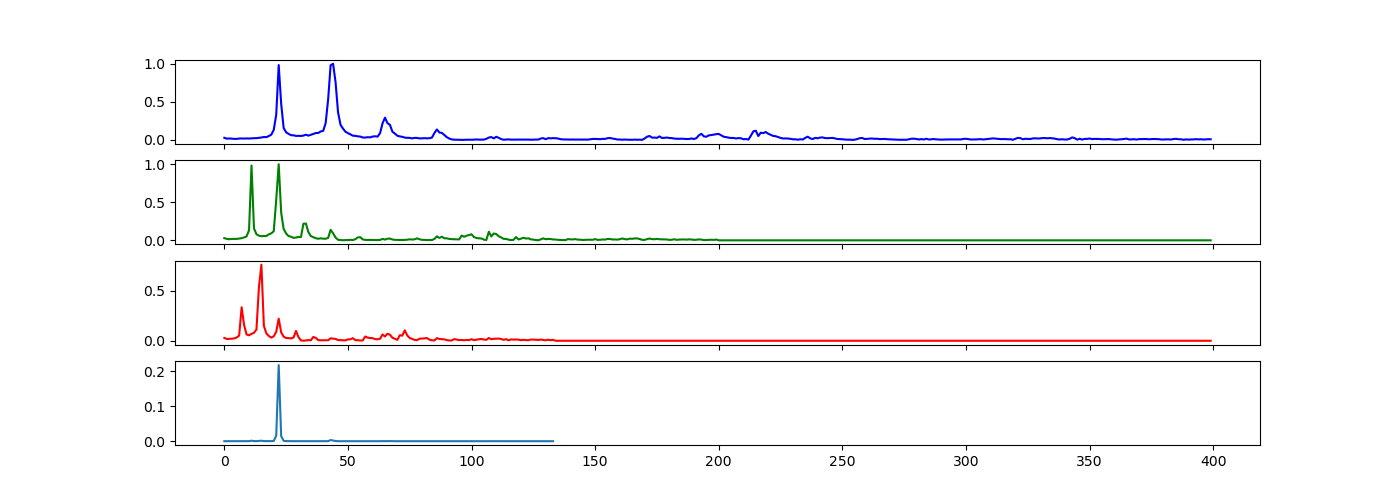
\includegraphics[width=\textwidth]{./images/hps.png}
    \caption{Plot of signal and downsampled versions of it and the final HPS. Harmonics align and form a peak. \label{fig:hps}}
\end{figure}

HPS is a good algorithm because it is simple and easy to compute making it suitable for real-time analysis. As the HPS essentially looks at the ratio of the harmonics, it can find a missing fundamental. Even if the fundemental is part of the spectrum, it may not always be the strongest in which case the HPS helps by enhancing it for easier discernment from noise.

The biggest problem with the HPS is that it does not perform well in the case of lacking harmonics \cite{McLeod2008}. This likely won't be a problem because human voices should be rich in harmonic content. In the more extreme case where noise is dominating, the system would still compute the HPS and one largest peak would form somewhere, resulting in garbage data. A possible way to mitigate this is to check the spectral flatness (sometimes called tonality) of the signal and ignore the results if over a certain threshold. Spectral flatness is usually defined as the ratio of the geometric mean and arithmetic mean of the power spectrum. This will be revisited in a later chapter. HPS is also prone to getting octaves wrong \cite{Smyth2019}.
% CFAR
\subsubsection{Constant False Alarm Rate}
% https://www.youtube.com/watch?v=BEg29UuZk6c
Constant False Alarm Rate (CFAR) is an algorithm that gives a dynamic threshold. It works by looking at some amount of reference cells that are beyond some gap around the target cell. For example for cells 5, 6, 7, 8, 9, 10, 11, 12, 13 the threshold given a gap size of 2 and reference cell count of 2 and the target is 9, the reference cells are 5, 6, 12 and 13. 7, 8, 10 and 11 are gap cells. The reference cells are then averaged (but other statistical methods can be used) and a bias may be applied. If the value of cell 9 is above the computed threshold, it is considered a target and noise if below. CFAR is typically used in conjunction with radar technology, but could just as well be used to discern the partials in a spectrum. 

\begin{figure}[ht]
    \centering
    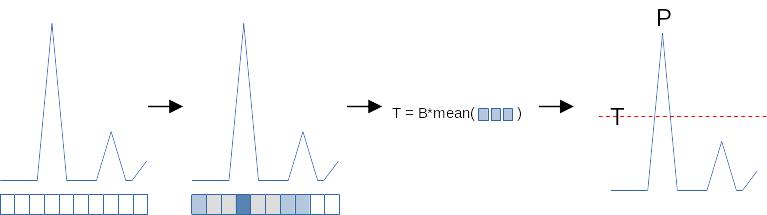
\includegraphics[width=\textwidth]{./images/cfar.png}
    \caption{Diagram of the CFAR algorithm with 2 gap cells and 2 reference cells. The gap cells around the target point P are excluded but the reference cells in light blue are used for calculations. The reference cells are averaged which gives the threshold T for point P. As P is greater than T, P is regarded as a target.\label{fig:cfar}}
\end{figure}

To effectively use CFAR, the parameters must be carefully chosen. If the bias is too low, invalid targets may be considered targets and vice versa if the bias is too high. The gap and reference cells can be fairly flexible but not too large, as smaller harmonics may be considered noise compared to greater harmonics. The lowest pitch we want to estimate is around 50Hz and if we assume monophonic singing, the spectrum should mostly contain integer multiples of the fundamental frequency which means that no peaks should ever be closer than 50Hz. With 4Hz bins, we can freely choose up to 12 gap and reference cells and not have a harmonic interfere with the CFAR computations of another. 

As CFAR only finds the peaks, one problem with using it alone as a fundemental frequency estimator is that additional post processing is necessary. Since HPS already works well for peak picking, it is chosen as the primary algorithm for the fundamental frequency estimator. CFAR could, however, be used to give a rough number for peaks, which may be used to dynamically adjust the number of iterations the HPS uses. If CFAR finds very few peaks or even just one as in the case of the electric piano in Figure \ref{fig:pianoFreq}, the result could be used to completely change peak picker as HPS has issues with signals without harmonics.

% Problems with FFT, might move this to real-time
\subsection{Problems with the FFT}
One problem with the FFT that \cite{Gotsopoulos} addresses is the size of the frequency bins. This is also noted for the STFT, limiting how short the STFT can be for achieving sufficient frequency resolution \cite{Evans2012}. The FFT doesn't find precise frequencies, it finds bins of frequencies with the size $S/N$ where $S$ is the sampling rate and $N$ is the FFT buffer size. As frequency grows exponentially (doubles every octave), higher notes are spaced further apart. This means that for lower notes, the frequency bins need to be significantly smaller as shown in Figure \ref{fig:fftBinSizeChart}. Base singers may need to go very low, around E2 (87Hz) and in order to avoid notes in this range to fall into the same bin, the window size needs to be very small.  

\begin{figure}[ht]
    \centering
    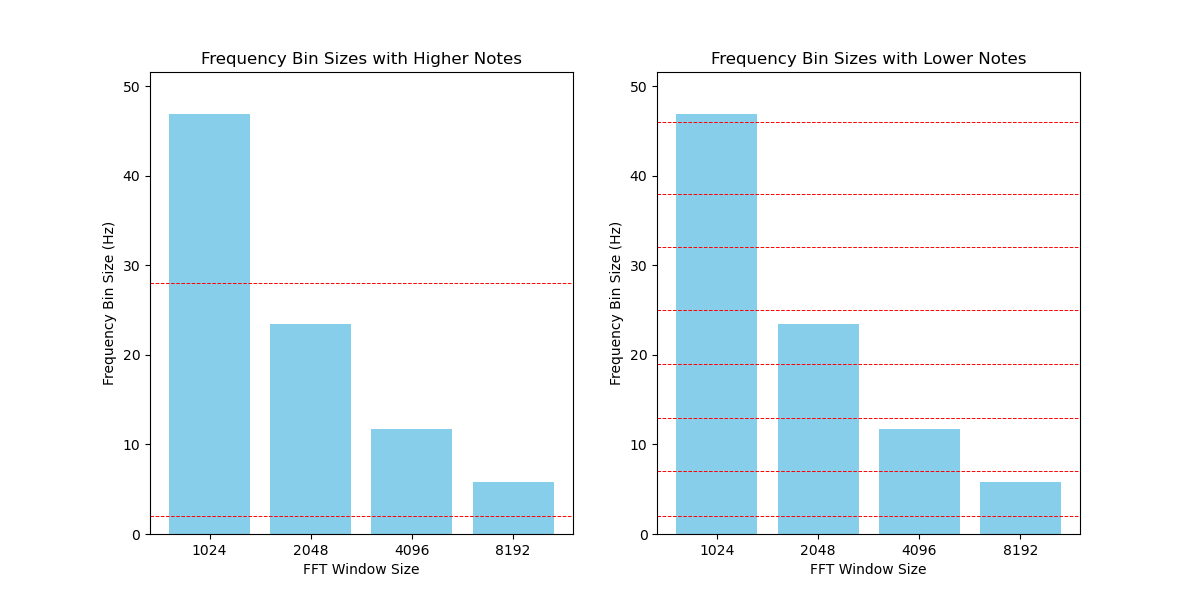
\includegraphics[width=\textwidth]{./images/fft_bin_size_chart.png}
    \caption{As the FFT window shrinks, different notes may fall into the same bin. Bars represent the bin sizes for various window sizes at 48kHz sampling rate and dashed lines show semitone intervals (the exact note values are irrelevant). For notes in the 4th octave, the window size can be smaller, but in the 2nd octave even 8192 samples is not enough to discern all pairs of semitones because the bins are larger than those semitone differences.\label{fig:fftBinSizeChart}}
\end{figure}

Base singers typically go as low as E2 and the difference between E2 and F2 is barely 5Hz which is smaller than the frequency bin of 8192 samples at 48kHz. They do not necessarily fall into the same bin but it would be safer to compute the FFT with a 16384 window size. This halves the frequency bin size and definitely accomodates differences even an octave lower. This introduces a significant amount of increased computation and is quite unnecessary as base singers do not realistically go much lower than E2. If the FFT implementation allows (many implementations require a power of 2), the window size should lie somewhere between 8192 and 16384 to lessen computations. For a 4Hz bin, $48000/x = 4 \iff x = 48000/4 = 12000$, 12000 samples would be enough to discern the lowest notes. 

This introduces another problem, which has implications for real-time pitch detection which is that collecting 12000 samples at 48kHz takes 0.25 seconds, which arguably is not real-time anymore. As the bin size is $B = S/W$ means that $W = S/B$ and the latency (time taken to fill the FFT window) $L = W/S = \frac{S/B}{S} = 1/B$, the bin size and latency are inversely proportional, both can not be minimized. For a bin size of 4, it will necessarily take 0.25s to collect the FFT samples. This follows that naively transforming audio makes real-time pitch detection for base singers impossible because the detection latency will inherently always be too long with sufficiently fine frequency resolution.

% Note timings
\subsection{Note lengths and timings}
Note lengths are defined as fractions in relation to the beat. The beat is the recurring pulse of the music which relates to the tempo and the time signature. In common time (which is noted with 4/4) the beat is implied to have the same length as a quarter note. A whole note thus is sustained over 4 beats and similarly two eight notes can be played in a single beat. Music is in other words always written using relative lengths and the overall speed is defined by the author often using natural language. The musician should respect the relative note lengths but they may or may not respect the pace set by the author.  


How a piece of music is performed often deviates considerably from how it was written. There are several reasons for this. For one, sheet music is not an algorithm but closer to natural language. There are many things that are up for interpretation, most notably as far as pace and dynamics are concerned. When a musician encounters the tempo marking, for example, \textit{andante}, they just have to know and/or feel what it means because there does not seem to be any consensus on what \textit{andante} means. Most sources give a range, but even the ranges are different between sources. Another term, \textit{accelerando} simply means to accelerate. By how much or how quickly is not specified. Musicians may ignore them completely and even make them up, to introduce their own touch into the performance. In the more simpler case, some sections may just be dragged as the musician or conductor wants. Figure \ref{fig:performance-sheet} visualizes two time series using color intensity instead of magnitude. This is for demonstration purposes only and how they were created is not of importance for the moment. The upper time series is the definition of the piece as the sheet music states. The time series below is one performance of the piece. The graphics reveals how the pace in the rendition deviates from the sheet. It should be easy to see a strong similarity between the two. They are not quite identical, but their structure is identical, and they have similar substructures. 

\begin{figure}[ht]
    \centering
    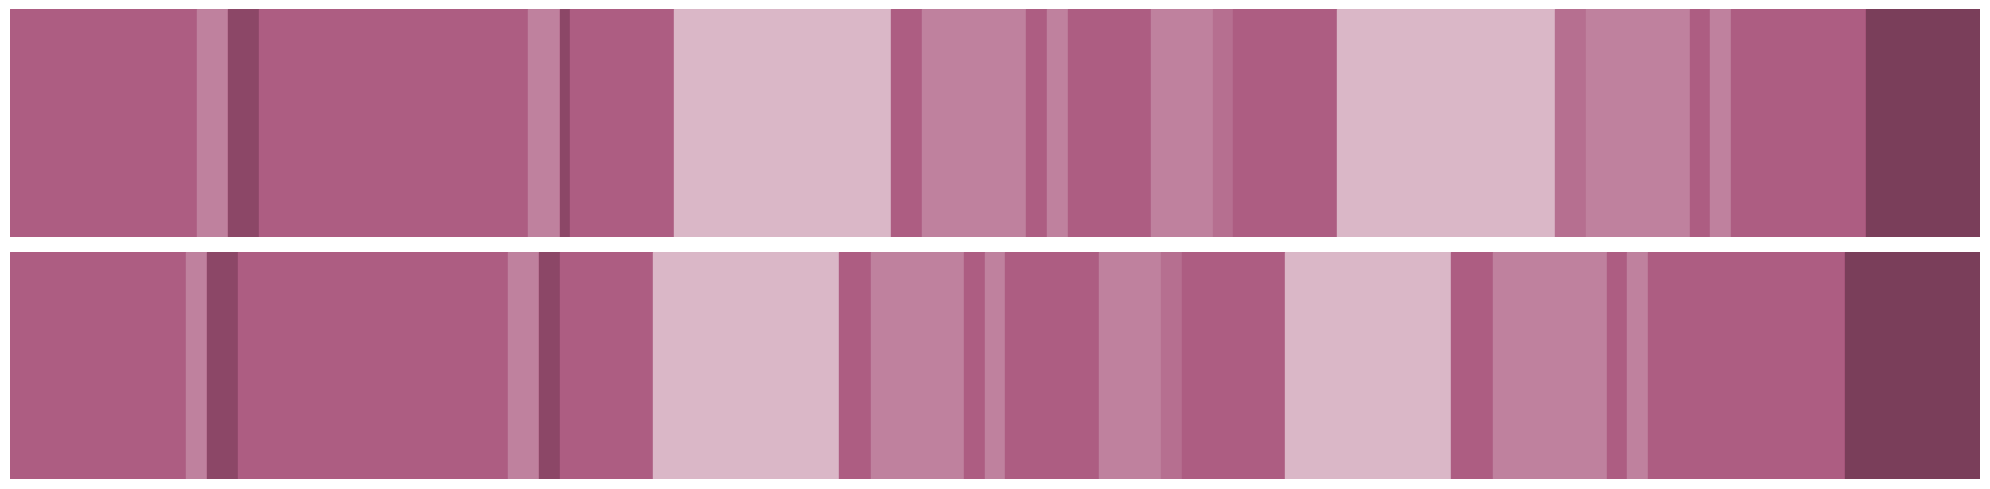
\includegraphics[width=\textwidth]{./images/performance-sheet.png}
    \caption{The time series of a piece as the sheet music suggests (above) and of a performance of said piece (below)\label{fig:performance-sheet}}
\end{figure}

\subsubsection{Time series similarity}
The similarity of two time series can be measured with Dynamic Time Warping. Timing and DTW is important to understand because it helps understanding the computational problems in creating the pitch detector. As DTW works with a longer signal (as opposed to a single sample), it is not suitable for real-time detection. DTW is thus used for developing and testing the detector using recordings for consistency and conveniance and is only a tool for the analysis of the notes detected by the pitch detector. 

% Narrowing the problem
\subsection{Real-time monophonic pitch detection}
The focus of this work is on real-time pitch detection, specifically for the purpose of rating and aiding a user in practicing their singing. To clarify, real-time means that the input of the system is a stream and the system processes small chunks as they come up and forget anything that it has already processed just like a human would listen to a short window in time, decide the pitch for that window and move on, not caring about the previous windows and not knowing anything of upcoming windows. The acceptable latency of \textit{real-time} is contextual. For rendering, it should be around 33 milliseconds to achieve 30 frames per second, where as for real-time tracking in logistics, it is probably enough to update every minute or even hour. 

What real-time means in this particular context can be debated and studied further but the goal is just that it is fast enough so that the user can react to their mistakes. This is akin to a teacher telling a student that they are off to give the student instant feedback, as opposed to saying something like “there was a mistake in the 3rd note in the 11th bar” which may be little to no help for a beginner. According to humanbenchmark.com, the mean reaction time is 284ms based on their collected 81M benchmarks \cite{HumanBenchmark2025}. The Human Benchmark benchmark is based on visual stimuli, but it is noted that the reaction to auditory stimuli is slightly faster \cite{SheltonKumar2010}. The goal for this work is significantly below the mean visual reaction time at around 100ms. In any case, even if humans can react to auditory stimuli faster than this, as the purpose is to give live feedback to the user on their own singing rather than having the user react to someone else's singing, the user is limited by their reaction speed to the feedback (which is visual stimuli).

% Zero padding
\subsubsection{Zero-padding}
One challenge with real-time pitch detection that emerged from the problem with the size of frequency bins was that for detecting lower base notes, the window size needed to be around 12000. However collecting 12000 samples at 48kHz takes 0.25s, which arguably is not real-time anymore. It takes 0.33s if for any reason the window size needs to be 16384. If the window size is made smaller, the resulting FFT will have larger bins than what is necessary for detecting lower frequencies. 

A popular approach to increasing frequency resolutions is to pad the end of the signal with zeros. Zero-padding makes the signal longer and while it necessarily introduces frequency components (more bins with a longer input signal), the peaks remain intact. A larger FFT window, while increasing computational complexity, allows for better frequency resolution. At 48kHz, 16000 samples are enough to achieve a 3Hz frequency bin. If out of these 16000, 10000 are zeros and 6000 legitimate datapoints, the FFT window can be "filled" in a mere 125ms which is a more acceptable latency for real-time detection. Figure \ref{fig:zeropadSpectrum} shows how zero-padding affects the spectrum.

\begin{figure}[ht]
    \centering
    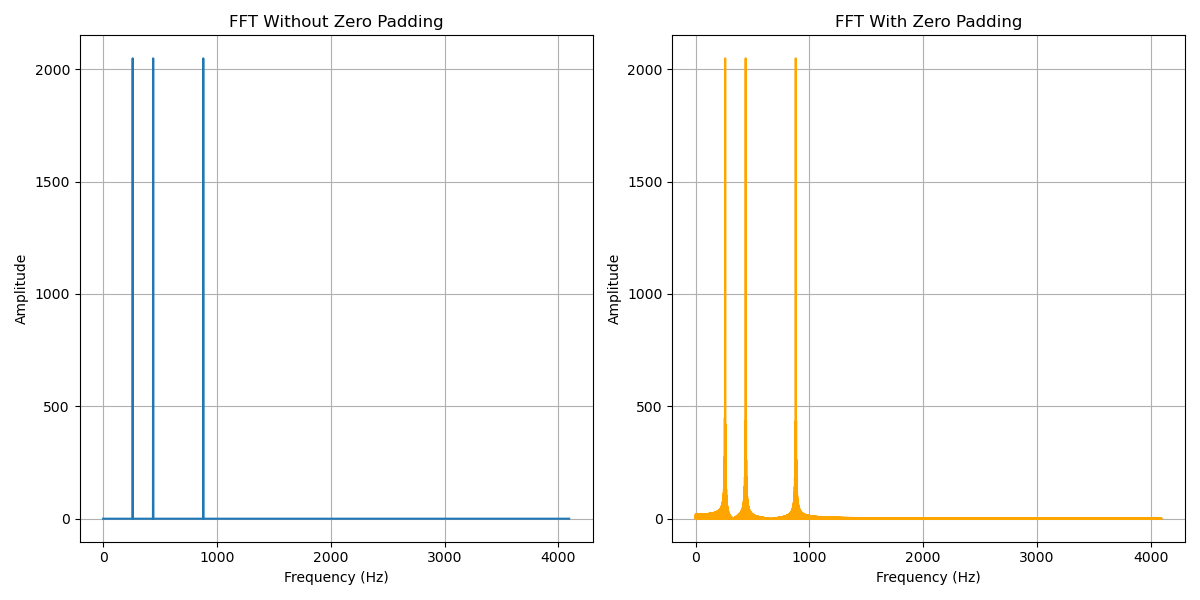
\includegraphics[width=\textwidth]{./images/zero_pad_spectrum.png}
    \caption{Spectrum contents of a signal consisting of 260, 440 and 880 frequency components. While the zero-padding introduces a small amount of frequency data around the peaks, the peaks themselves are not affected. \label{fig:zeropadSpectrum}}
\end{figure}

\subsubsection{Reducing sampling rate and window size}
As the bin size is the ratio of the sampling rate to number of samples, $B = S/N$, reducing both $N$ and $S$ keeps the bin size small. If only the window size is reduced, the bins grow in size and frequency resolution is lost. With zero-padding fixing the latency issue, why not reduce the sample rate as well to ease computational load? Apart from the system limitations of sampling rate, like the W3C web audio specifications only guaranteeing 8000 to 96000Hz, another issue is aliasing. Aliasing in short is misrepresentation of higher frequencies as lower frequencies. 

The Nyquist-Shannon sampling theorem states that there is no loss of imformation when sampling at 2B hertz if the signal contains frequency components that are less than B hertz. It thus implies that if we do lower the sampling rate, there will be some ambiguity about about the highest frequencies. For example, for the most common sampling rate 44100Hz, the maximum frequency that can be represented without ambiguity is 22050Hz. This is also called the Nyquist frequency. In other words, the Nyquist-Shannon theorem says that no information is lost as long as all frequency components are below the Nyquist frequency. 22050 being just above all frquencies humans can hear is a key factor for 44100Hz being the common default. 

As the pitch detector in this work has no reason to play back the sound, we can do whatever to with the waveform as long as no crucial information is lost or skewed. Compared to the lowest male voices, there's seems to be less consensus on the highest female voice, but a pitch higher than G6 at around 1567Hz see\ref{fig:performance-sheet}ms to be uncommon. A more typical is C6 at around 1046Hz. To be on the safe side, the 1567Hz can still be considered a valid requirement. If the pitch detector needs to detect a 1567Hz frequency, the sampling rate needs to be no smaller than 3134Hz. However, the human voice is rich in harmonics, if these are aliased, they will be presented as lower notes which in the best case would get the octave wrong and in the worst case get completely wrong notes.

The sampling theoren clearly states what we can and can not do with the signal but it all depends on the harmonics of voices. Clearly, the sampling rate can not be 3134Hz because a significant amount of the relevant information will be in the harmonics above 1567Hz, but from limited testing, the harmonics certainly don't approach the 22050 Nyquist frequency.  Even for female voices, the spectral content seems to be very weak above 10000Hz and almost indistinguishable from noise above 15000Hz. The sampling rate thus could probably be lowered to 30kHz or even 20kHz which would allow an FFT window size of 8192. This could be considered and tested if system resources were an issue, but a modern laptop is performant enough for a 16394 point FFT to not slow down the program.

\subsection{Finding nearest note}
%https://newt.phys.unsw.edu.au/jw/notes.html
Western tuning is done in equal temperaments, meaning the octave is evenly divided in 12. Using A4 (440Hz) as a reference, one can calculate every semitone's frequency with a signed index from A4 using the following function. 
$$f(i) = 2^{i/12}*440$$
For example the -2nd semitone using the formula is approximately G4 which indeed is 2 semitones under A4. To avoid negative indices, they can be shifted by some number. A4 is assigned the MIDI number 69 so this will be the number the scale gets shifted by. So to find the frequency of the i-th MIDI number the following function can be used.
$$f(i) = 2^{\frac{i-69}{12}}*440$$
To find a MIDI number based on frequency, the function can be rewritten as a function of $f$.
$$M(f) = 12*\log_2(f/440)+69$$
While the MIDI numbers are discrete, the derived formula interpolates between the MIDI numbers. If the input is a number that isn't a semitone, like 450, the result is $M(450) \approx 69.4$. This can be rounded to the nearest integer.

The function that will be used in the pitch detector is
$$M(f) = round(12*\log_2(f/440)+69)$$

\subsubsection{Octave shift for tenors}
Tenor's parts are written in a treble clef but sung an octave lower. This transposition is sometimes explicitly written with a little 8 under the clef sign, but in many cases this is not the case. This discrepancy is important to note when comparing the detected notes against the written notes. Some programs do encode the octave shift in the music XML when using the clef with the little 8 underneath, for instance, a C5 in the sheet music is in fact a C4 in the music XML. However, if it is missing, the user would be getting errors when singing correctly because the are always an octave too low. A simple solution would be to simply let the user decide if the octave shift should be applied or not as it can be difficult or downright impossible for a computer to 


\subsubsection{Time keeping}
How a piece is performed may deviate significantly from how it is written down by the author. If the purpose was offline processing, where the entire signal is given and the system processes it as fast as it can, DTW and other related processing tools may be used to rate the similarity of the performance and the how it is written to conclude how accurate the user's singing was. Here, the input is the user's entire performance/practice and they get back the complete analysis in one go. This won't necessarily take long because the performance penalty of the analysis is negligeable.

However, since the goal is to give live feedback to the user, to analyse any note, the system needs to know at all times what note it should be expecting. One easy approach is to just force the user into a steady tempo and perhaps have a metronome to help them keep the tempo. This way, the system can at a constant pace, iterate through all the expected notes and compare whatever it has to whatever it gets. This is both easy to implement and beneficial for the user because even though there is artistic freedom in music, tempo and keeping relative note lengths correct is still a vital skill. 

While the time series in \ref{fig:performance-sheet} illustrate a important point about relative time in music, the application will solve this by forcing the user to keeping a constant tempo which effectively aligns actual and expected notes, unless the user makes an error in time keeping. DTW will partially be used in testing the pitch detector because of recordings that were provided for this work by Finlands svenska manssångarförbund (FSM), an alliance of finland-swedish men's choirs. 

\section{Implementation}
\section{Analysis and discussion}

% Conclusions
\section{Conclusions}

% References
\bibliographystyle{IEEEtran}
\bibliography{references}

\end{document}